\newpage
\section{Introdução}
A Maratona de Programação é um evento da Sociedade Brasileira de Computação que existe desde o ano de 1996. A Maratona nasceu das competições regionais classificatórias para as finais mundiais do concurso de programação, o International Collegiate Programming Contest, e é parte da regional sulamericana do concurso.

Ela se destina a alunos e alunas de cursos de graduação e início de pós-graduação na área de Computação e afins (Ciência da Computação, Engenharia de Computação, Sistemas de Informação, Matemática, etc). A competição promove nos estudantes a criatividade, a capacidade de trabalho em equipe, a busca de novas soluções de software e a habilidade de resolver problemas sob pressão. De ano em ano temos observado que as instituições e principalmente as grandes empresas da área têm valorizado os alunos que participam da Maratona.

Várias universidades do Brasil desenvolvem concursos locais para escolher os melhores times para participar da Maratona de Programação. Estes times competem na Maratona (e portanto na regional sulamericana) de onde os melhores serão selecionados para participar das Finais Mundiais do evento. No ano de 2018, mais de 50 mil estudantes de mais de 3000 escolas de mais de 100 países competiram em regionais em todo o planeta, e apenas 135 (cerca de 1\%) participam das Finais Mundiais do evento, no Porto, Portugal. Seis times brasileiros, dos quase de 800 participantes, estarão presentes nas finais mundiais.

Os times são compostos por três estudantes, que tentarão resolver durante 5 horas o maior número possível dos 10 ou mais problemas que são entregues no início da competição. Estes estudantes têm à sua disposição apenas um computador e material impresso (livros, listagens, manuais) para vencer a batalha contra o relógio e os problemas propostos.

Os competidores do time devem colaborar para descobrir os problemas mais fáceis, projetar os testes, e construir as soluções que sejam aprovadas pelos juízes da competição. Alguns problemas requerem apenas compreensão, outros conhecimento de técnicas mais sofisticadas, e alguns podem ser realmente muito difíceis de serem resolvidos.

O julgamento é estrito. No início da competição os competidores recebem os problemas que devem ser resolvidos. Nos enunciados dos problemas constam exemplos dos dados dos problemas, mas eles não têm acesso às instâncias testadas pelos juízes. A cada submissão incorreta de um problema (ou seja, que deu resposta incorreta a uma das instâncias dos juízes) é atribuída uma penalidade de tempo. O time que conseguir resolver o maior número de problemas (no menor tempo acumulado com as penalidades, caso haja empate) é declarado o vencedor\footnote{Está introdução foi retirada do site oficial da Maratona de Programação. \url{http://maratona.ime.usp.br/}}. 

\subsection{Dicas para a competição}
Conforme você leu, a maratona de programação geralmente ocorre no período de 5 horas ininterruptas e seu objetivo é a resolução do maior número de problemas. Como a competição ocorre em um longo tempo lhe é aconselhável um preparo físico e mental para que você suporte o estresse da competição. Crie uma rotina de programação. Inicie com alguns minutos, passe para horas e logo você estará programando por horas a fio. Reuniões antes da competição com os integrantes do time auxiliam no entrosamento da equipe. Lembre-se sempre, está é uma competição em equipe. Não tente resolver tudo sozinho pois você irá perder tempo. Existem plataformas online que simulam a competição (também chamada de Contest) ou possuem um grande acervo de problemas relacionados a ela. Podemos mencionar algumas plataformas, tais como:
\begin{itemize}
    \item Codeforces
    \item URI Online Judge
    \item UVA Online Judge
\end{itemize}

Na maratona de programação cada problema tem uma cor relacionado a ele. Quando você consegue solucionar um problema lhe é dado o balão com a cor do problema. Utilize isso a seu favor. Quando a competição é iniciada procure olhar os `Standings' gerais. Busque resolver os problemas mais fáceis. Olhe ao redor e observe a frequência de aparição das cores, observe a figura \ref{fig:balao}. Este é o método mais fácil para descobrir se um problema é fácil ou não. Se nenhuma equipe conter a cor do balão associado ao exercício o qual você julga ser fácil, revise o problema pois ele pode não ser tão simples assim.

\begin{figure}[H]
    \caption{Balões Maratona de Programação}    
    \centering
    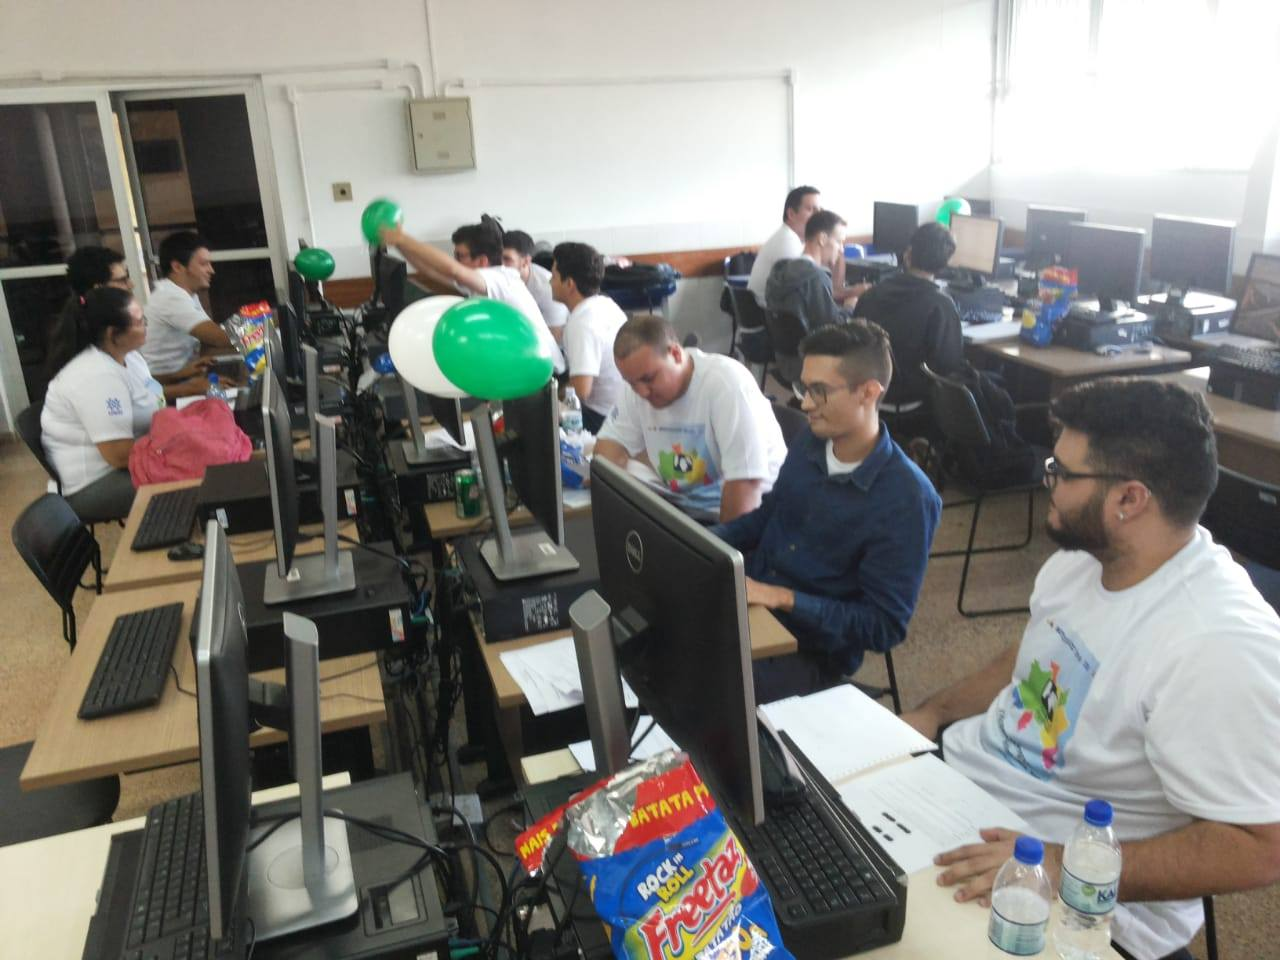
\includegraphics[scale = 0.2]{image/balao.jpg}
    \label{fig:balao}
\end{figure}
\begin{center}
    Fonte: Maratona de Programação do Norte, 2019.
\end{center}

Nas próximas seções serão abordados técnicas e problemas que comumente aparecem na competição e algumas das várias maneiras para aborda-los.

\subsection{Análise de Algoritmos}
A análise de algoritmo é peça fundamental na competição. Existem diversos problemas em que podemos facilmente acreditar que ele um problema é fácil. Porém, ao pensarmos que é um problema fácil acabamos por aborda-lo com uma solução \textit{naive} (ingênua) por não termos o conhecimento de análise de algoritmos. O objetivo da análise de algoritmos é estudar o melhor algoritmo possível para solucionar determinado problema.
Conforme a literatura explana, existem três tipos de notações assintóticas estudadas na computação. Sendo elas:

    \begin{itemize}
        \item $\Omega$ - Omega
        \item $\Theta$ - Theta
        \item O - Big O
    \end{itemize}
    
    Onde $\Omega$ é conhecido como o melhor caso possível, $\Theta$ caso médio, e O como pior caso. Abordaremos somente a notação Big O. Pois a análise via Big O nos permite encontrar o melhor algoritmo possível para o pior caso.
    
    Para que possa entender melhor o que é o Big O imagine o seguinte caso: 
    
    
    
\lstinputlisting[style=CPP,label={O(n)},caption = {Algoritmo O(n)}]{algoritmos/primeiro.cpp}
\vspace{1cm}
\rule{\textwidth}{0.4pt}
\large{\textbf{Exercícios\footnote{Os exercícios encontram-se disponíveis na plataforma URI Online Judge \url{htps://www.urionlinejudge.com.br}}}}\\

\begin{itemize}
    \item \textbf{1221} - Primo Rápido
    \item \textbf{1424} - Problema Fácil de Rujia Liu?
    \item \textbf{1805} - Soma Natural
\end{itemize}

\newpage